\documentclass{article}
\usepackage{amsmath}
\usepackage{array}
\usepackage{xspace}
\usepackage{color}
\usepackage{graphicx}
\usepackage{float} % utiliser H pour forcer a mettre l'image ou on veut
\usepackage{lscape} % utilisation du mode paysage
\usepackage{mathbbol} % permet d'avoir le vrai symbol pour les reels grace a mathbb
\usepackage{enumerate} % permet d'utiliser enumerate
\usepackage{marvosym} % permet d'avoir le symbol pour le nucleaire
\usepackage{moreverb} % permet d'utiliser verbatimtab : conservation la tabulation
\usepackage{stmaryrd} % permet d'utiliser \llbrackedt et \rrbracket : double crochet
\usepackage{caption}
\usepackage{subcaption}
\usepackage[noabbrev]{cleveref} % permet d'utiliser cref and Cref

\usepackage{setspace}
%\doublespacing

\setlength{\textwidth}{16.6cm}
\setlength{\textheight}{21cm}
\setlength{\oddsidemargin}{0cm}
\setlength{\headsep}{5pt} 

\newcommand\bn{\boldsymbol{\nabla}}
\newcommand\bo{\boldsymbol{\Omega}}
\newcommand\br{\mathbf{r}}
\newcommand\la{\left\langle}
\newcommand\ra{\right\rangle}
\newcommand\bs{\boldsymbol}
\newcommand\red{\textcolor{red}}
\newcommand\ldb{\{\!\!\{}
\newcommand\rdb{\}\!\!\}}
\newcommand\llb{\llbracket}
\newcommand\rrb{\rrbracket}
\newcommand\mc{\mathcal}

\renewcommand{\(}{\left(}
\renewcommand{\)}{\right)}
\renewcommand{\[}{\left[}
\renewcommand{\]}{\right]}

\newcommand{\sn}{\ensuremath{S_n}\xspace}
\newcommand{\tf}{b_i}

\newtheorem{algorithm}{Algorithm}[section]

% DGFEM commands
\newcommand{\jmp}[1]{\llb #1 \rrb}                     % jump
\newcommand{\mvl}[1]{\ldb #1 \rdb}             % mean value
%


\begin{document}
\title{Discontinuous Diffusion Synthetic Acceleration for Sn Transport on
2D Arbitrary Polygonal Meshes}
\author{} 
\date{}
\maketitle

\begin{abstract}
  \textcolor{red}{The Modified Interior Penalty (MIP) Diffusion Synthetic Acceleration (DSA) technique
  is extended to the Piece-Wise Linear Discontinuous (PWLD) finite elements.\\
	In this paper, the Diffusion Synthetic Acceleration (DSA) technique, based
	on the Modified Interior Penalty (MIP), is adapted to Piece-Wise Linear 
	Discontinuous (PWLD) finite elements.}\\
  This \textcolor{red}{provides/yields/results in} an efficient DSA preconditioner for arbitrary 
	polygonal/polyhedral meshes. 
	Such arbitrary grids (which include triangular and tetrahedral meshes as a subset) can be used to model complex objects; 
	they can also be advantageously employed 
	with locally refined spatial grids without the need to deal with ``hanging nodes''. 
  The MIP technique was originally derived to solve diffusion problems using discontinuous finite elements;
	it yields a system of linear equations that is 
  is Symmetric Positive Definite (SPD). Thus, solution techniques, such as Preconditioned 
	Conjugate Gradient (PCG), can be effectively employed. 
	In this research, we compare Symmetric Gauss-Seidel (SGS) and Algebraic MultiGrid (AMG) methods
	as preconditioners
  Fourier analyses are 
  performed for the MIP-DSA formulation using PWLD finite elements and we show that this scheme is
  always stable and effective at reducing the spectral radius for iterative transport
  solves, including for grids with high-aspect ratio cells.
  Numerical results are presented for different grids (quadrilateral, hexagonal, polygonal, and rectangular
	with local mesh adaptation). 
  AMG preconditioning for the MIP system is shown to be significantly more efficient 
  than SGS preconditioning.
\end{abstract}

%%%%%%%%%%%%%%%%%%%%%%%%%%%%%%%%%%%%%%%%%%%%%%%%%%%%%%%%%%%%%%%%%%%%%%%%%%%%%%%%%%
%%%%%%%%%%%%%%%%%%%%%%%%%%%%%%%%%%%%%%%%%%%%%%%%%%%%%%%%%%%%%%%%%%%%%%%%%%%%%%%%%%
\section{Introduction}
%%%%%%%%%%%%%%%%%%%%%%%%%%%%%%%%%%%%%%%%%%%%%%%%%%%%%%%%%%%%%%%%%%%%%%%%%%%%%%%%%%
%%%%%%%%%%%%%%%%%%%%%%%%%%%%%%%%%%%%%%%%%%%%%%%%%%%%%%%%%%%%%%%%%%%%%%%%%%%%%%%%%%

We present a Diffusion Synthetic Acceleration (DSA) scheme
that is fully compatible with the Piece-Wise Linear Discontinuous (PWLD) finite
element discretization of the transport equation on arbitrary
polygonal cells. 

Arbitrary polygonal (polyhedral in 3D) cells can advantageously be employed, especially
in the context of spatial discretizations based on discontinuous finite elements (DFE),
for the following reasons:
polygonal grids may allow for a reduced numbers of unknowns and/or can provide a natural
transition for locally adapted meshes. To illustrate these two points, first consider
a hexagonal cell. Employing a PWLD discretization, such a cell possesses six unknowns. Using
alternate DFE discretizations that perform well in the thick diffusive limit, such as 
linear discontinuous on triangles and bilinear discontinuous on quadrangles, the same 
hexagonal cell could be split into two quadrangles (for a total of 8 unknowns), two 
triangles and one quadrangle (10 unknowns), or four triangles (12 unknowns). By inserting an 
extra point inside the cell, the hexagon could also be divided into three quadrangles 
(12 unknowns), four quadrangles (16 unknowns) or six triangles (18 unknowns). A 
similar reasoning can be applied to any $n$-polygon. Arbitrary polygonal grids can 
also handle locally refined meshes in a natural manner. The example given
in \Cref{fig_amr} is typical of simulations performed with Adaptive Mesh 
Refinement (AMR). Solvers based on arbitrary polygonal cells can easily handle cells 
with various numbers of edges as follows: on \Cref{fig_amr}, the left cell is actually interpreted 
as a pentagon whereas the two cells on the right are quadrilaterals. PWLD spatial
discretization can handle locally adapted meshes without any special treatment 
or further approximation of the coupling between cells.
\begin{figure}[H]
   \centering
   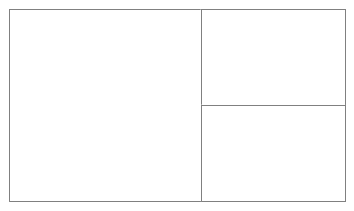
\includegraphics[width=0.3\textwidth]{amr.png}
   \caption{AMR mesh.}
   \label{fig_amr}
\end{figure}


%%%%%%%%%%%%%%%%%%%%%%%%%%%%%%%%%%%%%%%%%%%%%%%%%%%%%%%%%%%%%%%%%%%%%%%%%%%%%%%%%%
%\subsection{Rationale for DSA preconditioning}
%%%%%%%%%%%%%%%%%%%%%%%%%%%%%%%%%%%%%%%%%%%%%%%%%%%%%%%%%%%%%%%%%%%%%%%%%%%%%%%%%%

Next, we recall the rationale for diffusion acceleration schemes (preconditioners) 
\textcolor{red}{applied to the iterative solution of
transport problems (/ when solving iteratively transport problems).}
Because analytical solutions are unavailable for most
radiation transport problems of practical interest, one typically employs
iterative techniques to solve the large system of equations that results from
the spatial and angular discretizations of the transport equation. Standard
iterative techniques for the first-order form of the discrete-ordinate (\sn)
transport equation include the Source Iteration (SI) technique and Krylov 
subspace algorithms (usually GMRes \cite{gmres}). For highly diffusive materials 
(i.e., with scattering ratios $c=\Sigma_s / \Sigma_t $ close to 1) and optically 
thick configurations (i.e., problems that are not leakage-dominated), these iterative techniques 
can become quite ineffective, requiring high iteration counts and possibly 
leading to false convergence. To mitigate these issues, SI and GMRES-based transport solves 
can be effectively accelerated (preconditioned) using Diffusion Synthetic Acceleration (DSA) 
\cite{dsa_ref,larsen_dsa,consistent_p1,m4s,wla,mip}. 

The spatial discretization of the DSA equations
must be somewhat ``consistent'' with the one used for the \sn transport equations 
in order to yield unconditionally stable and efficient DSA schemes
\cite{dsa_ref,larsen_dsa,consistent_p1,m4s,wla,mip}. However, the search for full
consistency between the discretized transport equations and the discretized
diffusion may not be computationally practical (especially for unstructured
arbitrary meshes, \cite{dsa_ref}). For instance, Warsa, Wareing, and
Morel \cite{consistent_p1} derived a fully consistent DSA scheme for linear
discontinuous finite elements on unstructured tetrahedral meshes; their DSA
scheme yielded a $P_1$ system of equations which was found to be
computationally more expensive than partially consistent DSA schemes that are
based upon discretizations of a standard diffusion equation. Some partially 
consistent schemes have been analyzed for discontinuous finite element
(DFE) discretizations of the transport equation on unstructured meshes, for
example, the modified-four-step (M4S) scheme \cite{m4s}, the
Wareing-Larsen-Adams (WLA) scheme \cite{wla}, and the Modified Interior
Penalty (MIP) scheme \cite{mip}.

%%%%%%%%%%%%%%%%%%%%%%%%%%%%%%%%%%%%%%%%%%%%%%%%%%%%%%%%%%%%%%%%%%%%%%%%%%%%%%%%%%
%\subsection{PWLD discretization on arbitrary grids}
%%%%%%%%%%%%%%%%%%%%%%%%%%%%%%%%%%%%%%%%%%%%%%%%%%%%%%%%%%%%%%%%%%%%%%%%%%%%%%%%%%

%% Several discretization methods haven been developed for 
%% arbitrary polygonal meshes \cite{pwld_2d,pwld_3d,cfm_dfm,pwl_diffusion,
%% palmer_fe,mimetic,cell_centered_diff,palmer_proc,palmer_ane,wachspress,pwbld}.
%% In this work, we focus on the PWLD discretization because it was successfully
%% used to discretize the transport equation \cite{pwld_2d,pwld_3d}. This
%% discretization can be applied for any polygonal cells and the integrals
%% generated by this discretization can be easily computed analytically. 

To the authors' knowledge, no work is currently done to adapt the M4S 
technique to polygonal meshes. This is probably due to the fact
that M4S does not yield a Symmetric Positive Definite (SPD)
matrix and was found to be divergent for 3D tetrahedral meshes with linear 
discontinuous elements \cite{consistent_p1}. 
% 
Recent work to develop a DSA scheme for polygonal cells has mainly focused 
on adapting the WLA scheme to polygonal meshes
\cite{cfm_dfm,wla_pwl}. The WLA scheme is a two-stage process, where first a
diffusion solution is obtained using a {\em continuous} finite element
discretization and then a {\em discontinuous } update is performed cell-by-cell 
in order to provide an appropriate discontinuous scalar flux correction to the DFE transport 
solver. In \cite{consistent_p1}, the WLA scheme was
found to be a stable and effective DSA technique, though its efficiency
degraded as the problem became more optically thick and highly diffusive.
%
In this paper, we present an extension of the MIP technique to the
PWLD discretization technique for arbitrary polygonal meshes.
The MIP scheme is based on the standard Interior Penalty (IP) method for the
discontinuous discretization of diffusion equations. MIP was first derived in
\cite{mip}, where it was applied to triangular unstructured meshes (with
locally adapted cells). MIP does \textcolor{red}{not suffer from the same problems than WLA when the
problem becomes optically thick and highly diffusive} and, therefore, can be a
viable alternative to the WLA scheme. Because MIP produces an SPD matrix, it has been 
solved using a Preconditioned Conjugate Gradient (PCG), with symmetric successive 
over-relaxation method (SSOR) as preconditioner \cite{mip}. In this paper, we also analyze  
the effectiveness of algebraic multigrid methods (AMG) \cite{amg,amg_course} to precondition 
the MIP-DSA diffusion solve and we compare AMG with PCG+\textcolor{red}{SGS/SSOR}.
%Algebraic multigrid methods allow the use of multigrid techniques when no grid
%information is available or when the grid is unstructured. Instead of using a
%succession of grids based on the geometry of the problems, the ``grid levels''
%are based on properties of the matrix.

The remainder of this paper is organized as follows. In \Cref{sec_transport},
we briefly recall the \sn transport equation, its discontinuous finite element
discretization using the PWLD technique, and the Source Iteration iterative scheme. 
The MIP-DSA scheme is reviewed and extended to the PWLD discretization for arbitrary 
polygons in \Cref{sec_mip}. In \Cref{sec_amg}, we introduce the Algebraic MultiGrid (AMG) 
approaches used here: the ML package of Trilinos \cite{ml_guide} and the
AGMG (AGgregation-based algebraic MultiGrid) technique
\cite{agmg_guide,agmg,agmg2,agmg3}. In
\Cref{sec_res}, we present a Fourier analysis for the MIP-DSA scheme discretized with
PWLD and we compare the different AMG with preconditioned CG solver.
Conclusions are given in \Cref{sec_conc}.

%%%%%%%%%%%%%%%%%%%%%%%%%%%%%%%%%%%%%%%%%%%%%%%%%%%%%%%%%%%%%%%%%%%%%%%%%%%%%%%%%%
%%%%%%%%%%%%%%%%%%%%%%%%%%%%%%%%%%%%%%%%%%%%%%%%%%%%%%%%%%%%%%%%%%%%%%%%%%%%%%%%%%
\section{Discretization and Solution Techniques for the $S_n$ Transport Equation}\label{sec_transport}
%%%%%%%%%%%%%%%%%%%%%%%%%%%%%%%%%%%%%%%%%%%%%%%%%%%%%%%%%%%%%%%%%%%%%%%%%%%%%%%%%%
%%%%%%%%%%%%%%%%%%%%%%%%%%%%%%%%%%%%%%%%%%%%%%%%%%%%%%%%%%%%%%%%%%%%%%%%%%%%%%%%%%

We recall the \sn transport equations, the iterative techniques
employed to solve them, and discuss the PWLD discontinuous spatial
discretization for the transport equation with an emphasis on arbitrary
polygonal/polyhedral grids.

%%%%%%%%%%%%%%%%%%%%%%%%%%%%%%%%%%%%%%%%%%%%%%%%%%%%%%%%%%%%%%%%%%%%%%%%%%%%%%%%%%
\subsection{The \sn Transport Equations}
%%%%%%%%%%%%%%%%%%%%%%%%%%%%%%%%%%%%%%%%%%%%%%%%%%%%%%%%%%%%%%%%%%%%%%%%%%%%%%%%%%
Given an angular quadrature set $\{\bo_m,w_m\}_{1\leq m \leq M}$, the one-group
\sn transport equation with isotropic source and scattering is:
\begin{equation}
  \( \bo_m\cdot \bn + \Sigma_t(\br) \) \psi_m (\br) = \frac{1}{4\pi} \left( \Sigma_s
  (\br) \phi(\br) + S (\br) \right), \ \textrm{ for } \br \in \mc{D},\
  1 \leq m \leq M,
  \label{transport_sn}
\end{equation}
with $\psi_m(\br) = \psi(\br,\bo_m)$ the angular flux at position $\br$ in
direction $\bo_m$, $\Sigma_t$ and $\Sigma_s$ the total and scattering cross
sections, respectively, and $\mc{D}$ the spatial domain. The scalar flux is
defined and evaluated as follows:
\begin{equation}
  \phi(\br) \equiv \int_{4\pi} \psi(\br,\bo) d\bo \approx \sum_{m=1}^M w_m
  \psi_m (\br).
\end{equation}
For brevity, we assume only incoming boundary conditions, that is, $\psi_m(\br_b) =
\psi_m^{inc}(\br_b)$ for any point on the inflow boundary: $\br_b \in \partial \mc{D}_m^-
= \{\partial \mc{D} \textrm{ such that }\bo_m \cdot \bs{n}_b <0\}$, with
$\bs{n}_b = \bs{n}(\br_b)$ the outward unit normal vector at $\br_b$. 
\Cref{transport_sn} can be written in a compact form using operators:
\begin{align}
  & \bs{L} \Psi = \bs{M \Sigma}\Phi + S \equiv q, \label{L_Psi}\\
  &\Phi = \bs{D} \Psi, \label{Phi}
\end{align}
where $\Psi$ is the vector of angular fluxes, $\Phi$ the scalar flux,
$q$ is the total (scattering+external) source $\bs{L}$ is the streaming
operator, $\bs{\Sigma}$ is the scattering matrix, $\bs{M}$ is the
moment-to-direction operator, and $\bs{D}$ is the direction-to-moment
operator. $\bs{L} = diag(\bs{L}_1,\hdots,\bs{L}_m,\hdots,\bs{L}_M)$ is 
a diagonal operator; given a total source $q$, one can solve independently 
for the resulting angular
fluxes in all directions. The action of $\bs{L}^{-1}$ is often referred to as
a transport sweep when discontinuous spatial approximations are
employed because, for any direction $\bo_m$, the action of $\bs{L}_m^{-1}$ can
be obtained by traversing the mesh (i.e., sweeping) in a specific ordering of
the cells, thus requiring only to solve a small linear system of equations,
cell by cell. The order in which the elements are solved constitutes the graph
of the sweep; for brevity and because this is not the focus of this article,
we do not expand on situations where the graph presents dependencies
(cycles); in such a case, these dependencies can either be lagged within the
iterative procedure \cite{dgfem} or the solution vector consisting of the scalar 
flux is augmented by the angular fluxes that cause the cycle \cite{mip}.

%%%%%%%%%%%%%%%%%%%%%%%%%%%%%%%%%%%%%%%%%%%%%%%%%%%%%%%%%%%%%%%%%%%%%%%%%%%%%%%%%%
\subsection{Solution Techniques}
%%%%%%%%%%%%%%%%%%%%%%%%%%%%%%%%%%%%%%%%%%%%%%%%%%%%%%%%%%%%%%%%%%%%%%%%%%%%%%%%%%

\Cref{L_Psi,Phi} can be solved using the Source Iteration (SI) method (a
stationary iterative technique also known as Richardson iteration). The SI
techniques at the $\ell^{th}$ iteration is given by :
\begin{equation}
  \Phi^{(\ell+1)} = \bs{DL}^{-1} \(\bs{M\Sigma}\Phi^{(\ell)} + S\).
\end{equation}
Alternatively, a subspace Krylov method (usually GMRes) can be employed to
solve the system of equations:
\begin{equation}
  \(\bs{I} - \bs{DL}^{-1}\bs{M \Sigma}\) \Phi = \bs{DL}^{-1}S
\end{equation}
SI and GMRes-based transport solves require transport sweeps (action of $\bs{L}^{-1}$).
When the scattering ratio
$c=\frac{\Sigma_s}{\Sigma_t}$ tends to one in optically thick domains, the
number of SI and GMRes iterations can become large. To speed up convergence, a DSA
preconditioner is needed; this is further discussed in \Cref{sec_mip} for arbitrary 
polygonal grids. 

%%%%%%%%%%%%%%%%%%%%%%%%%%%%%%%%%%%%%%%%%%%%%%%%%%%%%%%%%%%%%%%%%%%%%%%%%%%%%%%%%%
\subsection{Discontinuous Finite Element Discretization on Arbitrary Grids}
%%%%%%%%%%%%%%%%%%%%%%%%%%%%%%%%%%%%%%%%%%%%%%%%%%%%%%%%%%%%%%%%%%%%%%%%%%%%%%%%%%

The domain $\mc{D}$ is partitioned into arbitrary polygons. For 
a given streaming direction $\bo_m$, the discontinuous finite
element formulation, on a given element $K$, is:
\begin{equation}
  -\int_{K} \(\psi_m \bo_m \cdot \bn \tf + \Sigma_t \Psi_m \tf \)\ d\br +
  \int_{\partial K^+} \bo_m \cdot \bs{n} \Psi_m \tf \ d\br = \int_{K} q\, \tf \ d\br +
  \int_{\partial K^{-}} |\bo_m \cdot \bs{n}| \psi_m^{\uparrow}\, \tf \ d\br,
  \label{transport_int}
\end{equation}
where $\tf$ represents a generic finite element basis function, $\partial K^{-}$ 
is the inflow face of element $K$, $\partial K^{+}$ is the outflow face of 
element $K$. The angular flux values on an inflow face, denoted by 
$\psi_m^{\uparrow}$ in \cref{transport_int}, are taken from the upwind neighbor 
element of that face.

Now, we define the basis functions, $\tf$, for the PWLD discretization. First, we
introduce a within-cell point $c$ inside the polygon in 2D. The coordinates 
of $c$ are weighted averages of the vertex coordinates:
\begin{equation}
  u_c = \sum_{i=1}^{N_V} \alpha_i u_i,
\end{equation}
where $u=x$ or $y$, $N_V$ is the number of vertices for the cell under
consideration, and the (positive) weights $\alpha_i$ are such that $\sum_{i=1}^{N_V} \alpha_i =1$. 
The basis function at vertex $j$ is defined by 
\cite{pwld_2d}:
\begin{equation}
  b_i(x,y) = t_i(x,y) + \alpha_i t_c(x,y),
\end{equation}
where $t_i(x,y)$ is a linear function such that $t_i(x,y)$ is unity at vertex
$i$ and zero at vertices $i-1$, $i+1$, and $c$. The $t_c(x,y)$ function is a ``tent''
function in the interior of the cell; it is unity at the within-cell point $c$
and zero at all the vertices of the cell. The number of PWLD basis functions is 
equal to the number of vertices in the polygon (i.e., $1 \le i \le N_v$). In this paper, the arbitrary
positive weights $\alpha_i$ are chosen to be $\frac{1}{N_V}$; for example, on a
quadrilateral cell, we employ $\alpha_i =\frac{1}{4}$. Finally, note that on
triangular cells, the PWLD basis functions reduce to the
standard Linear Discontinuous (LD) basis functions if $\alpha_i = \frac{1}{3}$. 
Given the definition of the PWLD
finite elements, it may seem complicated to build the elementary transport 
matrices on an arbitrary polygonal cell but the construction of such matrices
can be greatly simplified using the notion of ``sub-cells'', where a ``sub-cell'',
in 2D, is defined as the triangular cell linking an edge of the polygonal cell to its
within-cell point. Note that these ``sub-cells'' are never created as part of the 
polygonal grid; they are just \textcolor{red}{a simple implementation means of computing}
the elementary matrices of a polygonal cell by loop over its sub-cells. 

%%%%%%%%%%%%%%%%%%%%%%%%%%%%%%%%%%%%%%%%%%%%%%%%%%%%%%%%%%%%%%%%%%%%%%%%%%%%%%%%%%
%%%%%%%%%%%%%%%%%%%%%%%%%%%%%%%%%%%%%%%%%%%%%%%%%%%%%%%%%%%%%%%%%%%%%%%%%%%%%%%%%%
\section{DSA on arbitrary polygonal cells} \label{sec_mip}
%%%%%%%%%%%%%%%%%%%%%%%%%%%%%%%%%%%%%%%%%%%%%%%%%%%%%%%%%%%%%%%%%%%%%%%%%%%%%%%%%%
%%%%%%%%%%%%%%%%%%%%%%%%%%%%%%%%%%%%%%%%%%%%%%%%%%%%%%%%%%%%%%%%%%%%%%%%%%%%%%%%%%

%%%%%%%%%%%%%%%%%%%%%%%%%%%%%%%%%%%%%%%%%%%%%%%%%%%%%%%%%%%%%%%%%%%%%%%%%%%%%%%%%%
\subsection{DSA Solution Principle}
%%%%%%%%%%%%%%%%%%%%%%%%%%%%%%%%%%%%%%%%%%%%%%%%%%%%%%%%%%%%%%%%%%%%%%%%%%%%%%%%%%

As noted earlier, in thick diffusive configurations, standard iterative techniques 
applied to transport solves 
can be slowly converging. DSA can be employed to accelerate their convergence.
The idea behind synthetic acceleration is that the error between the (yet
unknown) transport solution and the current iterate can be estimated from a
computationally less expensive process, yielding a correction term to be added
to the current iterate in order to improve the next iterate. In DSA, a
corrective scalar flux contribution, $\delta \Phi$, is sought through the following 
diffusion solve, 
\begin{equation}
  \bs{A}\ \delta \Phi = \bs{\Sigma}\(\Phi^{(\ell+1/2)} - \Phi^{(\ell)}\).
\end{equation}
where the source term is a scattering term due to the
difference between the previous iterate scalar flux $\Phi^{(\ell)}$ and the
newest scalar flux, $\Phi^{(\ell+1/2)}$, obtained after a single transport sweep. 
The next scalar flux iterate is obtained by adding the scalar flux correction to
the scalar flux obtained after a transport sweep:
\begin{equation}
  \Phi^{(\ell+1)} = \Phi^{(\ell+1/2)}+\delta \Phi.
\end{equation}
$\bs{A}$ is the DSA matrix.
Ideally, $\bs{A}$ should be SPD (such that efficient iterative techniques can 
be employed in its linear solve) and easy to form (even on arbitrary grids).

%%%%%%%%%%%%%%%%%%%%%%%%%%%%%%%%%%%%%%%%%%%%%%%%%%%%%%%%%%%%%%%%%%%%%%%%%%%%%%%%%%
\subsection{Modified Interior Penalty DSA for polygons}
%%%%%%%%%%%%%%%%%%%%%%%%%%%%%%%%%%%%%%%%%%%%%%%%%%%%%%%%%%%%%%%%%%%%%%%%%%%%%%%%%%

Now, we discuss the Modified Interior Penalty as a DSA scheme for arbitrary polygons. 
This DSA scheme employs the same discontinuous finite elements used in the 
transport discretization for the discretization of the diffusion operator. 
MIP-DSA has been shown to be always stable for isotropic scattering on triangular 
cells \cite{mip}. The MIP diffusion solve is based on the standard Interior Penalty scheme (IP)
\cite{ip}, with an appropriately modified penalty term. Consider 
following diffusion update equation:
\begin{align}
  \left(-\bn \cdot \mathrm{D} \bn  + \Sigma_a \right) \delta \phi &= Q_0 &\textrm{ for }\br \in
  \mc{D}\\
  \frac{1}{4}\delta \phi - \frac{1}{2} \mathrm{D} \partial_n \delta \phi & = 0 &\textrm{ for }
  \br \in \partial \mc{D} %^d \\
  %-\mathrm{D} \partial_n \phi &= J^{inc} & \textrm{ for } \br \in \partial
  %\mc{D}^r,
\end{align}
where $\mathrm{D}$ is the diffusion coefficient, $\Sigma_a$ is the absorption cross section, 
%$\partial \mc{D}^d$ is the
%boundary of the domain with Dirichlet condition, $\partial \mc{D}^r$ is the
%boundary of the domain with reflective condition, 
$Q_0=\Sigma_s\(\Phi^{(\ell+1/2)}-\Phi^{(\ell)}\)$, 
%$J^{inc} = \sum_{\bo_m\cdot\bs{n}_b >0} w_m 
%|\bo_m \cdot \bs{n}_b| \delta \psi_d$, 
and $\partial_{n_e} = \bs{n}_e\cdot \bn$ where
$\bs{n}_e$ is the normal unit vector associated with a given edge $e$ (on the
boundary $\bs{n}_e = \bs{n}_b$). 
%The only difference between IP and MIP is the
%penalty factor $\kappa_e^{IP}$ used for IP is replaced by a new penalty factor
%$\kappa_e^{MIP}$. Therefore, 
The weak form of MIP-DSA equations is given by:
\begin{equation}
a(\delta \phi,\phi^*) = l(\phi^*)
\label{mip}
\end{equation}
%
with:
\begin{equation}
\begin{split}
a(\delta \phi,\phi^*) =& \(\Sigma_a \delta \phi,\phi^*\)_{\mc{D}}+
  (\mathrm{D}\bn\delta \phi,\bn\phi^*)_{\mc{D}} + \(\kappa_e^{MIP} \llb\delta \phi\rrb,
\llb\phi^*\rrb\)_{E_h^i} + \(\llb\delta \phi\rrb,\ldb\mathrm{D}\partial_n
\phi^*\rdb\)_{E_h^i} +\\
& \(\ldb\mathrm{D}\partial_n \delta \phi\rdb,\llb\phi^*\rrb\)_{E_h^i} +
\(\kappa_e^{MIP}
\delta \phi,\phi^*\)_{\partial \mc{D}^d} -\frac{1}{2} \(\delta \phi,\mathrm{D} \partial_n
\phi^*\)_{\partial \mc{D}^d} - \frac{1}{2}\(\mathrm{D}\partial_n
\delta \phi,\phi^*\)_{\partial \mc{D}^d}
\label{mip_b}
\end{split}
\end{equation}
%
and
%
\begin{equation}
l(\phi^*) = (Q_0,\phi^*)_{\mc{D}}+ (J^{inc},\phi^*)_{\partial \mc{D}^r} .
\label{mip_l}
\end{equation}
%
The notations used are as follows:
$(f,g)_{\mc{D}} = \sum_{K\in \mathbb{T}_h} \(f,g\)_K$, with the element integrals defined as 
$(f,g)_K = \int_K fg\ d\br$; $(f,g)_{E_h^i}=\sum_{e\in E_h^i}(f,g)_e$, with the edge integrals defined as 
$(f,g)_e = \int_e fg\ ds$. In the above, 
 $\mathbb{T}_h$ denotes the partition of domain
$\mc{D}$ into non-overlapping elements $K$, $E_h^i$ is the set of interior
edges, $\delta \phi$ is the numerical solution for the diffusion correction and $\phi^*$ is any test function.
Any entry $A_{ij}$ of matrix $\bs{A}$ is simply: $A_{ij}= a(b_j,b_i)$. Matrix $\bs{A}$ is SPD
and thus can be solved using a preconditioned conjugate gradient technique.
%$\in W_{\mc{D}}^h$, $W_{\mc{D}}^h=\{P \in
%L^2(\mc{D}); P|_{K}\in V_p(K), \forall K \in \mathbb{T}_h\}$, where $V_p(K)$
%is the space of polynomials of degree up to $p$ on element $K$,  
%
The jump and mean value of a variable $u$  at the interface between two elements is defined as follows:
\begin{equation}
\llb u \rrb = u^+ - u^- \text{ and } \ldb u\rdb = \frac{u^+ + u^-}{2} ,
\end{equation}
respectively.
%
The definition of the left/right values along a given edge $e$ is
\begin{equation}
u^{\pm}= \lim_{s\rightarrow 0^{\pm}}u(\bs{r}+s\bs{n}_e) .
\end{equation}
%
The MIP penalty coefficient is given by
\begin{equation}
\kappa_e^{MIP} = \max\(\kappa_e^{IP},\frac{1}{4}\)
\end{equation}
with:
\begin{equation}
\kappa_e^{IP} = \left\{
\begin{aligned}
&\frac{c}{2} \frac{\mathrm{D^+}}{h_{\bot}^+} + \frac{c}{2}
\frac{\mathrm{D}^-}{h_{\bot}^-} & \textrm{on interior edges, i.e., }
e\in E_h^i\\
&c \frac{\mathrm{D}}{h_{\bot}} & \textrm{on boundary edges, i.e., } e
\in\partial \mc{D} %^d 
\end{aligned}
\right. 
\end{equation}
where $c$ is a constant (chosen to equal 4 here) and $h_{\bot}$ is the length of the cell in the direction
orthogonal to the edge $e$. 
%MIP yields only a correction for the scalar flux
%but by assuming that the angular dependence satisfies a diffusion expansion,
%the angular correction can be computed using:
%\begin{equation}
  %\varepsilon_d = \frac{1}{4\pi}(\phi-3\mathrm{D}\bn\phi\cdot \bo_d)
%\end{equation}
%This correction can be used when some of the boundary conditions are periodic
%or reflective.
%
When PWLD finite elements are employed, there is no 
simple way to compute $h_{\bot}$. To estimate $h_{\bot}$, we 
assume that the polygonal cells do not deviate too much from regular polygons. 
In such case, if the cell has an even number of edges, the orthogonal 
length equals two times the apothem, i.e., two times the segment between the 
midpoint of a side of the polygon and the center of this polygon 
$\(\textrm{apothem}=2\times \frac{\textrm{area}}{\textrm{perimeter}}\)$. 
\textcolor{red}{I think you mean area and perimeter of the triangle formed by the edge $e$ and polygon the mid-point. Confirm.}
If the cell has an odd number of edges, the orthogonal length is given by the 
apothem plus the circumradius, i.e., the radius of the circle circumscribed to 
the polygon $\(\textrm{circumradius}=\sqrt{\frac{2\times \textrm{area}}{N_V
\sin\(\frac{2\pi}{N_V}\)}}\)$. A summary of the definitions used for $h_{\bot}$ for 
any polygon as a function of the number of vertices is given in
\Cref{table_h_bot}.
\begin{table}[H]
  \begin{center}
    \caption{Orthogonal length $h_{\bot}$ for different polygons.}
    \begin{tabular}{|c|c|c|c|c|}
      \hline
      Number of vertices & 3 & 4 & $> 4$ and even & $> 4$ and odd \\
      \hline
      $h_{\bot}$ & $2 \times \frac{\textrm{area}}{L_e}$ &
$\frac{\textrm{area}}{L_e}$ & $4\times
\frac{\textrm{area}}{\textrm{perimeter}}$ & $2 \times
      \frac{\textrm{area}}{\textrm{perimeter}}+\sqrt{\frac{2\times
      \textrm{area}}{N_V\sin\(\frac{2\pi}{N_V}\)}}$\\
      \hline
    \end{tabular}
    \label{table_h_bot}
  \end{center}
\end{table}

%%%%%%%%%%%%%%%%%%%%%%%%%%%%%%%%%%%%%%%%%%%%%%%%%%%%%%%%%%%%%%%%%%%%%%%%%%%%%%%%%%
%%%%%%%%%%%%%%%%%%%%%%%%%%%%%%%%%%%%%%%%%%%%%%%%%%%%%%%%%%%%%%%%%%%%%%%%%%%%%%%%%%
\section{MIP-DSA Solves Based on Algebraic Multigrid Techniques} \label{sec_amg}
%%%%%%%%%%%%%%%%%%%%%%%%%%%%%%%%%%%%%%%%%%%%%%%%%%%%%%%%%%%%%%%%%%%%%%%%%%%%%%%%%%
%%%%%%%%%%%%%%%%%%%%%%%%%%%%%%%%%%%%%%%%%%%%%%%%%%%%%%%%%%%%%%%%%%%%%%%%%%%%%%%%%%

%%%%%%%%%%%%%%%%%%%%%%%%%%%%%%%%%%%%%%%%%%%%%%%%%%%%%%%%%%%%%%%%%%%%%%%%%%%%%%%%%%
\subsection{AMG Principles}
%%%%%%%%%%%%%%%%%%%%%%%%%%%%%%%%%%%%%%%%%%%%%%%%%%%%%%%%%%%%%%%%%%%%%%%%%%%%%%%%%%

As mentioned above, a common way to solve a SPD system of equations is to use a 
conjugate gradient technique preconditioned  with Symmetric Gauss-Seidel (PCG-SGS)
or SSOR (PCG-SSOR); SGS is simply SSOR with a damping factor of one. In this research, we
will compare the calculation time and the number of iterations using conjugate 
gradient preconditioned with Symmetric Gauss-Seidel (PCG-SGS) to those of CG preconditioned with an
algebraic multigrid method. PCG-SGS was chosen because little difference was noted 
when employing other damping factors for MIP-DSA on triangular grids \cite{wang_personal_comm}. 
An algebraic multigrid method was employed to precondition the Krylov solver for the 
even-parity finite element-spherical harmonics (FE-$P_N$) method; see, for instance,
\cite{amg_pn}. In \cite{amg_pn}, the use of AMG  as a 
preconditioner resulted in a 60\% reduction in the solution time compared to 
ILU(0) preconditioning and even more reduction compared to SSOR preconditioning. 
In our implementation, we have linked our code with the ML package 
\cite{ml_guide} of the Trilinos library and with the AGMG library \cite{agmg_guide}. 
ML is a multigrid preconditioning package that uses a smoothed aggregation 
algebraic multigrid to build a preconditioner for a Krylov method. AGMG is an 
aggregation-based algebraic multigrid library written in Fortran 90.
%
The first multigrid methods developed were geometric multigrid techniques, used as 
stand-alone solvers. In many applications, they achieve the so-called 
``textbook multigrid efficiency'', i.e., ``the solution to the governing 
system of equations [is attained] in a computational work that is a small 
multiple of the operation counts associated with discretizing the system'' 
\cite{textbook_eff}. However, in many other applications, multigrid methods, 
and particularly algebraic multigrid methods, cannot achieve such efficiency, 
\cite{k_cycle} and, in such cases, they are often used as preconditioner for 
Krylov subspace methods. 

Before describing a general multigrid method, we recall the process using a 
two-grid method. Consider the following system
\begin{equation}
  \bs{A}_f u_f = b_f,
\end{equation}
defined on a fine grid $\Gamma_f$. The two-grid algorithm is as follows:
\begin{enumerate}
  \item Perform $\nu_1$ pre-smoothing iterations using a smoother (Jacobi,
    Gauss-Seidel, or ILU) and an initial guess $u_0$: $u = S^{\nu_1}(u_0,b_f)$
  \item Compute the residual on the fine grid $\Gamma_f$ and restrict it to
    the coarse grid $\Gamma_c$: $r_c = \bs{R}(b_f-\bs{A}_f u)$;
  \item Solve the system on the coarse grid: $v=\bs{A}_c^{-1} r_c$;
  \item Interpolate the coarse grid correction to the fine grid and add the
    correction to $u$: $u=u+\bs{P}v$;
  \item Perform $\nu_2$ post-smoothing iterations: $u = S^{\nu_2}(u,b_f)$.
\end{enumerate}
When using AMG, the matrix $\bs{A}_c$ on the coarse grid is given by the
Galerkin approximation:
\begin{equation}
  \bs{A}_c = \bs{R} \bs{A}_f \bs{P},
\end{equation}
where $\bs{P}$ is a prolongation matrix and $\bs{R}$ is a restriction matrix. 
Generally, solving the system $\bs{A}_c v = r_c$ on the coarse grid is still
quite expensive, therefore this step is recursively replaced by $n_{\gamma}$
sequences of the two-grid method until the system can be efficiently inverted 
with a direct solver.
%This yields the multigrid method. 
When $\gamma = 1$, respectively $\gamma =
2$, the multigrid method is said to use a $V-$cycle, respectively a $W-$cycle. 
\Cref{fig_v_w} shows typical $V-$ and $W-$ cycles. In \Cref{fig_v_w}, a 
dot represents a smoothing operation and a square a
direct inversion; the grid transfer operators are symbolized by the line segments.
\begin{figure}[H]
  \centering
  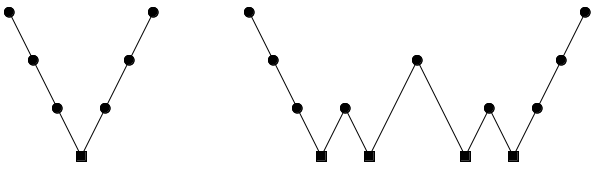
\includegraphics[width=0.5\textwidth]{v_w_cycles}
  \caption{$V-$ and $W-$cycles.}
  \label{fig_v_w}
\end{figure}

The main difference between geometric and algebraic multigrid techniques
lies in the method used
to coarsen the grid. Algebraic multigrid methods only use the properties of the
matrix. Among the algebraic multigrid methods, there are three main categories: 
the classical Ruge-Stueben AMG, the plain aggregation AMG, and the
smoothed aggregation AMG. ML uses smoothed aggregation AMG and AGMG
uses plain aggregation AMG. Next, we briefly explain the coarsening step in
the ML and AGMG implementations. The coarsening step is the most important 
step because if the coarsening occurs too fast, convergence rates will 
decrease. However, if coarsening is too slow, more memory may be 
required to solve the problem. 

%%%%%%%%%%%%%%%%%%%%%%%%%%%%%%%%%%%%%%%%%%%%%%%%%%%%%%%%%%%%%%%%%%%%%%%%%%%%%%%%%%
\subsection{The ML Package of Trilinos}
%%%%%%%%%%%%%%%%%%%%%%%%%%%%%%%%%%%%%%%%%%%%%%%%%%%%%%%%%%%%%%%%%%%%%%%%%%%%%%%%%%
When using a smoothed aggregation scheme, the smoothed interpolation operators
$\bs{P}_k$ are the transpose of the coarsening operators
$\bs{R}_k=\bs{P}_k^T$. Therefore, when the $\bs{P}_k$ matrices are built, the
coarsening operator is also known. First, the graph of the matrix is
constructed: if element $(i,j)$ or $(j,i)$ of the matrix is non-zero, an edge
is built between the vertex $i$ and the vertex $j$ \cite{ml_guide}. Second,
the vertices are 
aggregated. When using ML on a single processor, two aggregation schemes can
be used: the uncoupled scheme or the maximally independent sets (MIS) scheme. 
The uncoupled scheme tries to build aggregates of size $3^d$ where $d$ is the
dimension of the problem; its algorithm proceeds as follows \cite{mis}:
\begin{description}
  \item[Step 1:] As long as there are points not adjacent to an aggregate:
    \begin{enumerate}
      \item Choose a point which is not an adjacent to an
        aggregate. This point is a new root point.
      \item Define a new aggregate as the root point and its neighbors 
    \end{enumerate}
  \item[Step 2:] Add all the points left to the existing aggregates or form 
    new aggregates with them.
\end{description}
The MIS scheme used in ML applies the MIS algorithm \cite{graph_coloring} to
the graph of the matrix $\bs{A}^2$. These two coarsening 
schemes use a fixed ratio of coarsening between levels. 
%
Once aggregation is done, a tentative prolongation matrix, $\bs{\tilde{P}}_k$ 
is constructed \cite{mis}. A example of $\bs{\tilde{P}}_k$ is given by:
\begin{equation}
  \bs{\tilde{P}}_k(i,j) = \left\{
  \begin{aligned}
    &1 &\textrm{if the }i^{th}\textrm{ point is contained in the }j^{th}\textrm{
    aggregate}\\
    & 0 &\textrm{otherwise}
  \end{aligned}
  \right.
\end{equation}
This tentative prolongation operator could be used as is but smoothing it
allows to have a more robust scheme. Let $\bs{S}_k$ be a smoother, for example
damped Jacobi. Then, the prolongation matrix is given by:
\begin{equation}
  \bs{P}_k = \bs{S}_k \bs{\tilde{P}}_k.
\end{equation}

%%%%%%%%%%%%%%%%%%%%%%%%%%%%%%%%%%%%%%%%%%%%%%%%%%%%%%%%%%%%%%%%%%%%%%%%%%%%%%%%%%
\subsection{The AGMG Package}
%%%%%%%%%%%%%%%%%%%%%%%%%%%%%%%%%%%%%%%%%%%%%%%%%%%%%%%%%%%%%%%%%%%%%%%%%%%%%%%%%%
Unlike in ML, the prolongation operator in AGMG is not smoothed; this results in a
cheaper setup and a decrease in memory requirements \cite{agmg2}. However,
such a scheme could be less robust. To counteract this weakness, the
aggregation scheme is more involved. Coarsening algorithms that control
the size of the aggregates tend to produce a few badly shaped aggregates.
Since the convergence of AMG is bounded by the worst aggregate, even a small 
number of badly shaped aggregates can have a huge impact on
the convergence. In AGMG, the aggregation algorithm has as input the upper
bound of the two-grid condition number. When the aggregates are constructed,
their quality is checked. Obviously, this increases the cost of the coarsening
and it is thus important that the coarsening is fast enough. Such an 
algorithm does not control the size of the aggregates, and, therefore, it is 
difficult to control the speed of coarsening. However, controlling the condition 
number rather than the coarsening speed \textcolor{red}{can be a potent alternative approach}. By 
monitoring the condition number, bad aggregates will not be created and, instead, 
a few aggregates below the target size may be generated. This  
does not affect the efficiency of the method in a noticeable way \cite{agmg2}. 
A simple way to create the aggregates would be to try to exhaust all of the possible 
combinations, compute their quality, and then choose the optimal
coarsening. In practice, this would be too costly, and, in AGMG, the aggregation 
step is done by a few passes of a pairwise aggregation algorithm. Each pass
aggregates the variables two by two to allow a simple computation of the aggregate 
quality and to keep the cost per iteration low. The advantage of controlling the 
condition number becomes even more important when a $K-$cycle, or Krylov-cycle, is 
used instead of the more common $V-$ or $W-$cycles. The difference between the 
$K-$cycle and the $V-$ or $W-$cycles is that $K-$cycles use a 
few iterations of a Krylov solver preconditioned by a coarser grid to solve 
the coarse grid problem in the two-grid algorithm \cite{k_cycle}. The
advantage of the $K-$cycle is an increased robustness compared to $V-$ and
$W-$cycle. This scheme 
is nonlinear and requires, when the system is SPD, the use of flexible CG 
\cite{fcg,fcg_2,fcg_3,fcg_4} as the Krylov solver. Even when the condition 
number of the two-grid method is large, the convergence properties of the 
$K-$cycle can be independent of the number of levels \cite{k_cycle}. The 
computational cost of the $K-$cycle is about the same than that of a $W-$cycle. 
If the number of unknowns does not decrease sufficiently from one 
level to the next, the $K-$cycle at one level is replaced by a $V-$cycle at 
this level. At that level, no Krylov solver is used in order to decrease the
computational cost of the method. 

%\textcolor{red}{so what is used?}

%%%%%%%%%%%%%%%%%%%%%%%%%%%%%%%%%%%%%%%%%%%%%%%%%%%%%%%%%%%%%%%%%%%%%%%%%%%%%%%%%%
%%%%%%%%%%%%%%%%%%%%%%%%%%%%%%%%%%%%%%%%%%%%%%%%%%%%%%%%%%%%%%%%%%%%%%%%%%%%%%%%%%
\section{Results} \label{sec_res}
%%%%%%%%%%%%%%%%%%%%%%%%%%%%%%%%%%%%%%%%%%%%%%%%%%%%%%%%%%%%%%%%%%%%%%%%%%%%%%%%%%
%%%%%%%%%%%%%%%%%%%%%%%%%%%%%%%%%%%%%%%%%%%%%%%%%%%%%%%%%%%%%%%%%%%%%%%%%%%%%%%%%%

In this section, we present two series of results. First, Fourier analyses are 
carried out to analyze the performance of the MIP-DSA acceleration scheme 
for an homogeneous infinite medium meshed with rectangular cells and discretized with PWLD.
The effects of the $S_n$ order and the cell aspect ratio on the spectral radius of the iterative 
scheme are also studied. Second, the MIP-DSA technique is implemented in a 2D \sn code that uses
arbitrary polygonal grids with a PWLD spatial discretization.  Numerical examples employ
several meshes: arbitrary quadrilaterals, arbitrary polygons, a regular layout of 
hexagons/triangles/rectangles, and a grid that mimics adaptive mesh refinement 
performed on rectangular cells. The MIP-DSA diffusion solves are performed using various
linear solvers: Conjugate Gradient (CG), Conjugate Gradient
Preconditioned with Symmetric Gauss-Seidel (PCG-SGS), Conjugate Gradient
Preconditioned with ML using Uncoupled aggregation (PCG-ML/U),
Conjugate Gradient Preconditioned with ML using MIS aggregation (PCG-ML/MIS),
and Conjugate Gradient Preconditioned AGMG (AGMG). 

%%%%%%%%%%%%%%%%%%%%%%%%%%%%%%%%%%%%%%%%%%%%%%%%%%%%%%%%%%%%%%%%%%%%%%%%%%%%%%%%%%
\subsection{Fourier Analyses}
%%%%%%%%%%%%%%%%%%%%%%%%%%%%%%%%%%%%%%%%%%%%%%%%%%%%%%%%%%%%%%%%%%%%%%%%%%%%%%%%%%

Fourier analyses are often performed to assess some of the properties of 
DSA-accelerated transport solves \cite{larsen_dsa,consistent_p1,more}. In a Fourier analysis,
the eigenvalues of the iteration matrix are analyzed, assuming a Fourier ansatz for the 
error modes \cite{}. For instance, the iteration matrices for the SI and SI+DSA schemes are given by
\begin{equation}
\bs{D L^{-1}M \Sigma} \quad \text{and} \quad \bs{I}-\bs{(I+A^{-1}\Sigma)(I-D L^{-1}M \Sigma)},
\end{equation}
respectively. \textcolor{red}{check that} The error modes are of the form $\exp(i \bs{\Lambda} \cdot \bs{r})$, with the
wave number $\bs{\Lambda}=[\lambda_x,\, \lambda_y]^T$. The expressions for these modes 
are inserted into the discretized equations and the spectral radius (largest eigenvalue in magnitude)
of the iteration matrices are sought for $0 \le \lambda_x \le 2\pi/X$ and $0 \le \lambda_y \le 2\pi/Y$,
where $X$, and $Y$ are the dimensions of the rectangular domain.


\subsubsection{Spectral radius as a function of the $S_n$ order}
%%%%%%%%%%%%%%%%%%%%%%%%%%%%%%%%%%%%%%%%%%%%%%%%%%%%%%%%%%%%%%%%%%%%%%%%%%%%%%%%%%

This Fourier analysis is carried on a square cell ($X=Y$), using a
Gauss-Legendre-Chebyshev (GLC) angular quadrature. The medium is homogeneous with a 
scattering ratio $c=0.9999$; periodic boundary conditions are used. The results 
are plotted on \Cref{fig_fa_sn}, where the $x-$axis is the mesh size in mean free 
paths and the $y-$axis is the spectral radius. There are four curves corresponding 
to different $S_n$ orders: $S_2$, $S_4$, $S_8$ and $S_{16}$.
From \Cref{fig_fa_sn}, we conclude that MIP is stable for every 
cell size. The spectral radius is always less than 0.5, except for $S_2$ where 
it is about 0.7. In the fine mesh limit, the spatial continuum results are recovered:
the spectral radius of SI+DSA using an $S_2$ quadrature in 2D is $0.5c$; as the angular 
quadrature is refined, the standard result of $0.2247c$ for the spectral result is obtained.
\begin{figure}[!htbp]
  \centering
  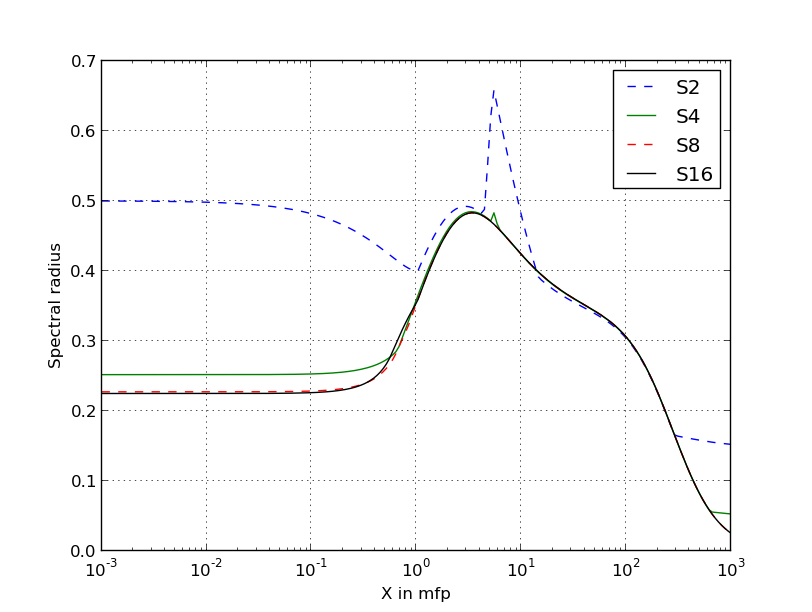
\includegraphics[width=0.7\textwidth]{sn_order_9999}
  \caption{Fourier analysis as a function of the mesh optical thickness, square cell,
    various \sn orders.}
  \label{fig_fa_sn}
\end{figure}

\subsubsection{Spectral radius as a function of the cell aspect ratio}
%%%%%%%%%%%%%%%%%%%%%%%%%%%%%%%%%%%%%%%%%%%%%%%%%%%%%%%%%%%%%%%%%%%%%%%%%%%%%%%%%%
For this Fourier analysis, we use a $S_{16}$ GLC quadrature. The medium is
again homogeneous with $c=0.9999$ and periodic boundary conditions apply. 
On \Cref{fig_fa_ar}, the five curves correspond to the following cell aspect 
ratios: $\frac{Y}{X}=\frac{1}{16}$, $\frac{Y}{X}=\frac{1}{4}$,
$\frac{Y}{X}=1$, $\frac{Y}{X}=4$, $\frac{Y}{X}=16$, and $\frac{Y}{X}=100$.
We note that the MIP-DSA scheme is stable for every aspect ratio tested, including 100, 
and that the maximum spectral radius shows little sensitivity to the aspect ratio.
\begin{figure}[!htbp]
  \centering
  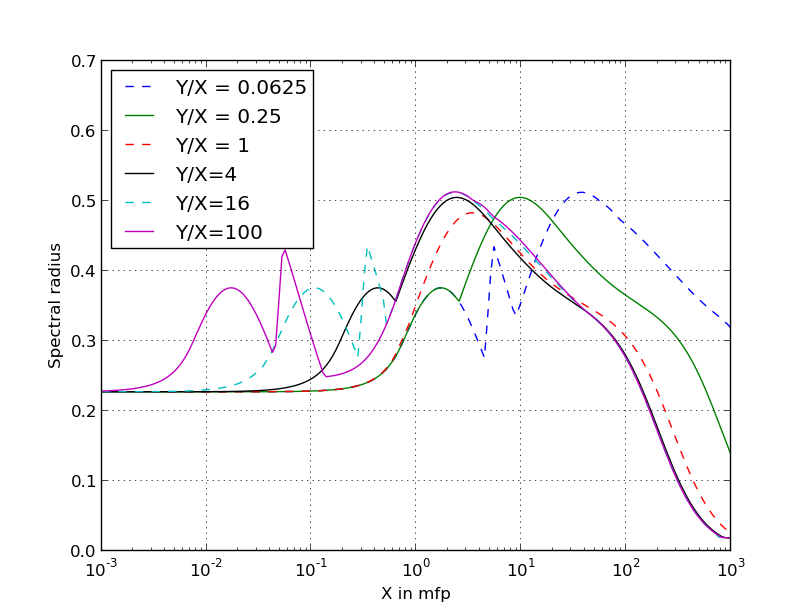
\includegraphics[width=0.7\textwidth]{aspect_ratio_9999_2}
  \caption{Fourier analysis as a function of the mesh optical thickness,
  $S_{16}$ angular quadrature, various aspect ratios.}
  \label{fig_fa_ar}
\end{figure}

%%%%%%%%%%%%%%%%%%%%%%%%%%%%%%%%%%%%%%%%%%%%%%%%%%%%%%%%%%%%%%%%%%%%%%%%%%%%%%%%%%
\subsection{Performance of MIP-DSA Implemented in a PWLD $S_n$ Transport Code}
%%%%%%%%%%%%%%%%%%%%%%%%%%%%%%%%%%%%%%%%%%%%%%%%%%%%%%%%%%%%%%%%%%%%%%%%%%%%%%%%%%
The MIP-DSA scheme has been implemented in a 2D \sn code that employs a PWLD discretization
for arbitrary polygonal grids. Several test cases are presented.

\subsubsection{Homogeneous test problems}  \label{sec_homog}
%%%%%%%%%%%%%%%%%%%%%%%%%%%%%%%%%%%%%%%%%%%%%%%%%%%%%%%%%%%%%%%%%%%%%%%%%%%%%%%%%%

We compare the different linear solvers employed for MIP-DSA using a homogeneous medium, $100cm
\times 100cm$, $\Sigma_t = 1cm^{-1}$ and $\Sigma_s = 0.999cm^{-1}$, with
vacuum boundary conditions and a unit source of intensity $1cm^{-3}s^{-1}$. We
use an $S_8$ GLC angular quadrature, Source Iteration as solver
with relative tolerance of $10^{-8}$ and a relative tolerance of
$10^{-10}$ for MIP-DSA solver. The medium is discretized using two different meshes:
\begin{enumerate}
  \item a quadrilateral gridcomposed of 49263 quadrilateral
    cells (197,052 degrees of freedom); 
  \item a polygonal grid composed of 45,204 triangles, 823
    quadrilaterals, 4,978 pentagons, 4,155 hexagons, 725 heptagons, and 24
    octagons, for a total of 55,909 cells and 193,991 degrees of freedom. This
    example will allow us to test MIP and the different preconditioners on a
    mesh composed of different cell types.
\end{enumerate}
%
The meshes and the numerical solutions are given on \Cref{homog_test}.
In \Cref{comparison_homog_quad}, results obtained with the different linear solvers for MIP-DSA 
are compared for the quadrilateral grid.
In \Cref{comparison_homog_quad}, SI iterations is the number iterations of 
needed to solve the problem, Precond init is the time, in
seconds, needed to initialize the preconditioner used by CG, MIP calculation
is the total time, in seconds, spent solving DSA during the calculation, CG
iterations is the total number of CG iterations used to solve MIP, and Total
calculation is the time, in seconds, needed to solve the problem. 
We note that the accelerated transport solves only require 24 SI iterations, regardless of the linear solver
employed in MIP-DSA (as expected). Preconditioning CG significantly reduces the number of CG iterations.
%
We observe that algebraic multigrid processes, PGC-ML and AGMG, require 
about the same number of iterations (two orders of magnitude less than unpreconditioned CG). 
However, AMG is significantly faster than PCG-ML. We also note that PCG-SGS iteration is 
slower than one unpreconditioned CG iteration. Profiling of the code reveals that the
bottleneck is the function \emph{Ifpack\_PointRelaxation::ApplyInverseSGS\_FastCrsMatrix} 
of Trilinos. This function applies the forward and the backward substitutions required by SGS.
It is unclear why these substitutions are so costly. Also note that SGS is employed as
a pre- and post-smoother in the ML package of Trilinos and the same function
is once again the bottleneck of the method.
%
The different linear solvers are compared for the polygonal grid in \Cref{comparison_homog_poly}:
We note that using different spatial cell types in the same grid does not affect
the performance of MIP-DSA or that of its preconditioners.

\textcolor{red}{why is the min value in the colorbar different for these 2 grids??? The grids seem refined enough ....}

\textcolor{red}{also, add the vtk to the repo in case I would like to do a zoom in to better show the quadrilateral/polygonal cells}
%
\begin{figure}[!htbp]
  \centering
  \begin{subfigure}{0.75\textwidth}
    \centering
    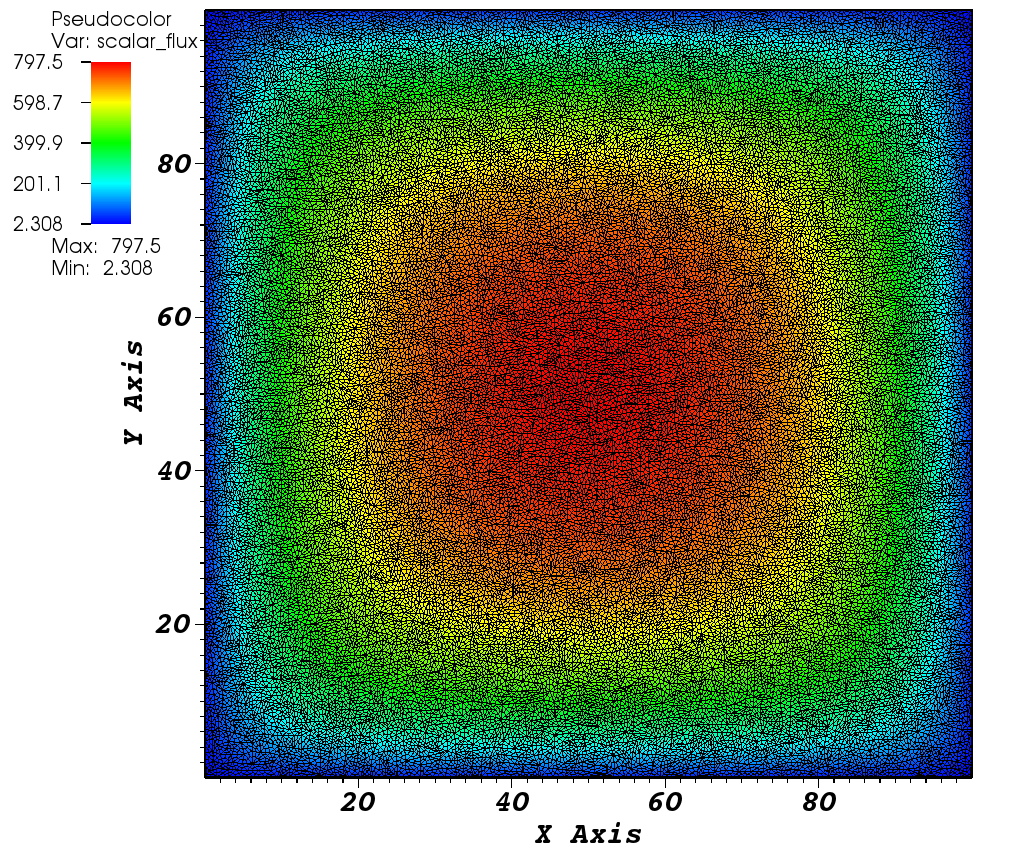
\includegraphics[width=\textwidth]{big_homog_quad_crop}
    \caption{Quadrilateral cells}
  \end{subfigure}
  \begin{subfigure}{0.75\textwidth}
    \centering
    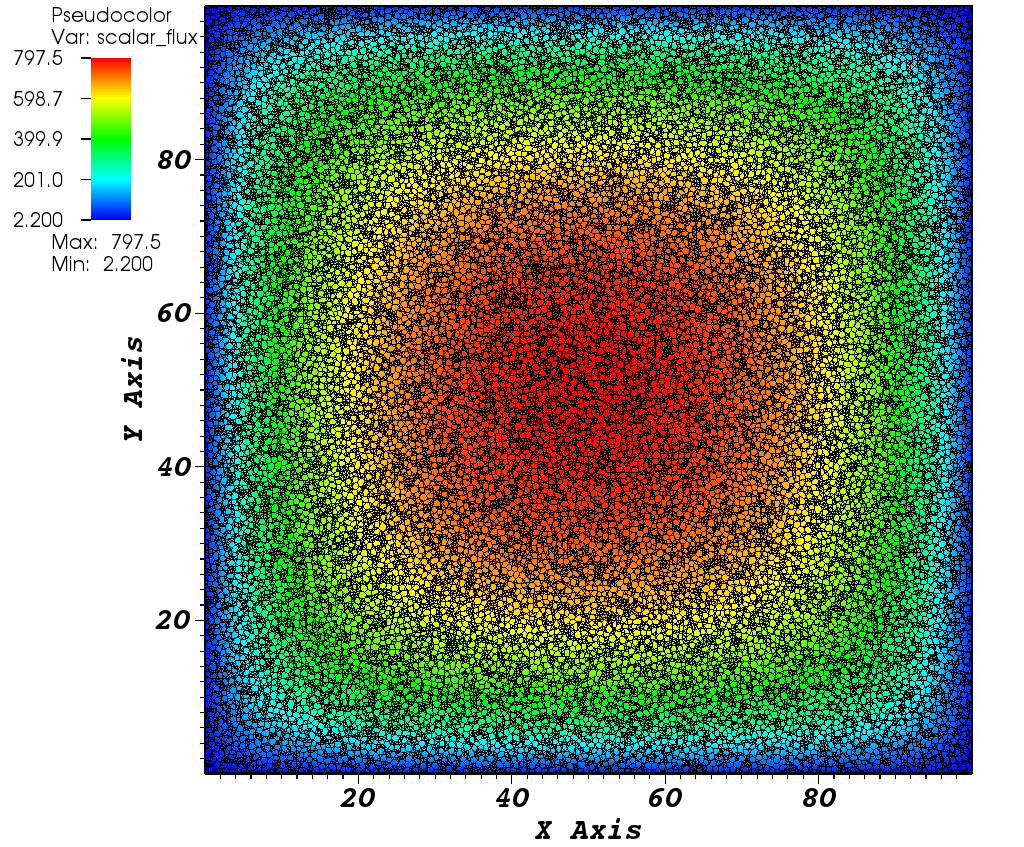
\includegraphics[width=\textwidth]{big_homog_poly_crop}
    \caption{Polygonal cells}
  \end{subfigure}
  \caption{Grids and scalar flux solutions for the homogenous material test problem}
  \label{homog_test}
\end{figure}
%
\begin{table}[!htbp]
  \begin{center}
    \caption{Comparison of different preconditioners for quadrilateral cells}
    \begin{tabular}{|c|c|c|c|c|c|c|}
      \hline
      & No-DSA & CG & PCG-SGS & PCG-ML/U & PCG-ML/MIS & AGMG \\
      \hline
      SI iterations   & 7311    & 24      & 24       & 24      & 24      & 24 \\
   Precond init (s)   & NA      & NA      & 0.171358 & 1.8255  & 9.56078 & 0.332 \\
MIP calculation (s)   & NA      & 1095.7  & 1311.76  & 192.622 & 197.632 & 29.9727 \\
      CG iterations   & NA      & 56649   & 17332    & 630     & 604     & 578 \\
Total calculation (s) & 39176.7 & 1264.98 & 1477.95  & 363.202 & 367.841 &
      194.568 \\
      \hline
    \end{tabular}
    \label{comparison_homog_quad}
  \end{center}
\end{table}
%
\begin{table}[!htbp]
  \begin{center}
    \caption{Comparison of different preconditioners for polygonal cells}
    \begin{tabular}{|c|c|c|c|c|c|c|}
      \hline
      & No-DSA & CG & PCG-SGS & PCG-ML/U & PCG-ML/MIS & AGMG \\
      \hline
      SI iterations   & 7311    & 23      & 23      & 23      & 23      & 23 \\
   Precond init (s)   & NA      & NA      & 0.06388 & 1.73379 & 8.0426  & 0.388 \\
MIP calculation (s)   & NA      & 877.861 & 1263.31 & 198.63  & 191.989 &
      31.242 \\
      CG iterations   & NA      & 46262   & 16712   & 652     & 603     & 555 \\
Total calculation (s) & 42666.7 & 1060.53 & 1447.53 & 382.275 & 384.422 &
      216.946 \\
      \hline
    \end{tabular}
    \label{comparison_homog_poly}
  \end{center}
\end{table}

\subsubsection{Heterogeneous medium}
%%%%%%%%%%%%%%%%%%%%%%%%%%%%%%%%%%%%%%%%%%%%%%%%%%%%%%%%%%%%%%%%%%%%%%%%%%%%%%%%%%

\textcolor{red}{why not make this problem thick? DSA is almost useless ....\\}
\textcolor{red}{also, add the vtk to the repo in case I would like to do a zoom in to better show the cells}

In this example, a heterogeneous geometry with three materials is used. It is 
composed of 184 triangles, 3,720 quadrilaterals and 2,791 regular hexagons of 
side $0.05cm$ for a total of 6,695 cells and 32,178 degrees of freedom (spatial 
unknowns per angular direction). The domain is $5.28275cm$ by $4.6cm$. 
Reflective boundary conditions are used. A $S_{16}$ GLC 
quadrature is used. The SI solver has a relative tolerance of 
$10^{-8}$ and the relative tolerance for MIP is $10^{-10}$. \Cref{hex_zones}
shows the problem geometry and the material properties are in given
\Cref{hex_prop}.
The different linear solvers for MIP-DSA are compared in \Cref{comparison_hex}.
%
\begin{figure}[!htbp]
  \centering
  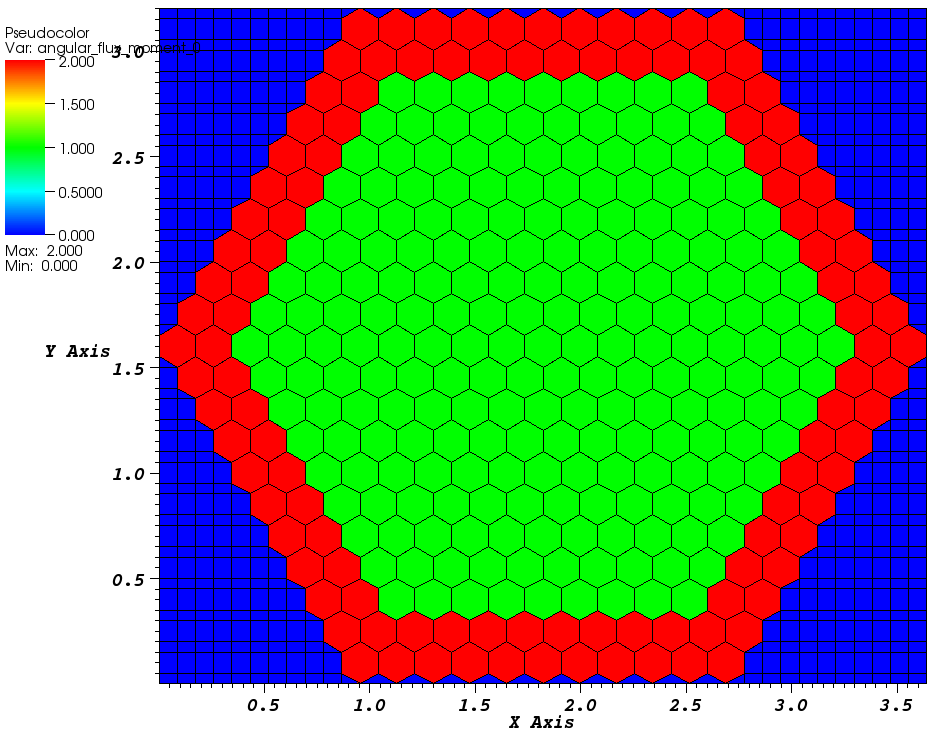
\includegraphics[width=0.6\textwidth]{source_crop}
  \caption{Material zones for the heterogeneous test problem}
  \label{hex_zones}
\end{figure}
%
\begin{table}[!htbp]
  \begin{center}
    \caption{Properties of the different zones}
    \begin{tabular}{|c|c|c|c|}
      \hline
       & Inner region & Intermediate region & Outer region \\
      $\Sigma_t$ $(cm^{-1})$ & 1.5 & 1.0 & 1.0 \\
      $\Sigma_s$ $(cm^{-1})$ & 1.4999 & 0.999 & 0.3 \\
     source $(cm^{-3}s^{-1}$ & 1.0 & 0.0 & 0.0 \\
      \hline
    \end{tabular}
    \label{hex_prop}
  \end{center}
\end{table}
%
%
\begin{table}[!htbp]
  \begin{center}
    \caption{Comparison of preconditioners, heterogeneous problem}
    \begin{tabular}{|c|c|c|c|c|c|c|}
      \hline
      & No-DSA & CG & PCG-SGS & PCG-ML/U & PCG-ML/MIS & AGMG\\
      \hline
      SI iterations & 278     & 17      & 17        & 17       & 17      & 17  \\
   Precond init (s) & NA      & NA      & 0.0160661 & 0.368768 & 1.41632 &
      0.07  \\
MIP calculation (s) & NA      & 58.422  & 126.93    & 33.2225  & 31.3045 &
      2.924 \\
      CG iterations & NA      & 12214   & 6679      & 415      & 386     & 248  \\
Total calculation (s) & 910.566 & 120.889 & 190.413 & 99.7524  & 97.4666 &
      70.6424 \\      
      \hline
    \end{tabular}
    \label{comparison_hex}
  \end{center}
\end{table}
%
The remarks made in \Cref{sec_homog} for the homogeneous test problem
remain mostly unchanged. MIP-DSA is effective for this heterogeneous test case and AGMG is
still the fastest solver. It is interesting to note that, contrary to the
homogeneous tests where the number of CG iterations remained similar for all
algebraic multigrid preconditioners, in this test, AGMG requires
significantly fewer iterations than the Trilinos implementations, PCG-ML/U and and PCG-ML/MIS.

\subsubsection{Locally refined grid}
%%%%%%%%%%%%%%%%%%%%%%%%%%%%%%%%%%%%%%%%%%%%%%%%%%%%%%%%%%%%%%%%%%%%%%%%%%%%%%%%%%

\textcolor{red}{also, add the vtk to the repo in case I would like to do a zoom in to better show the cells}

%\cite{mip}
In this example, a 3-material domain of size $10cm\times 10cm$ is used. 
\Cref{mat_amr} shows the material zoning and the mesh used. Material properties 
are given in \Cref{prop_amr}. The grid used mimics meshes obtained via adaptive mesh
refinement: the rectangular cells at the interfaces between two materials are refined once more,
leading to a grid composed of 10,482 quadrilaterals, 236 pentagons,
and 2 hexagons for a total of 10,720 cells and 43120 degrees of freedom. The bottom
and left sides of the domain have reflective boundary conditions, while the other two sides
have vacuum boundary conditions. 
%
The distribution of cells is given \Cref{fig_pol_dist}.
A $S_{16}$ GLC quadrature is employed. The tolerance on SI is $10^{-8}$ and
the tolerance on the CG solvers is $10^{-10}$.
The different linear solvers for MIP-DSA are compared in \Cref{table_amr}.
%
The conclusions drawn from this test case are similar to the ones made for 
our previous tests. This test case demonstrates that degenerate polygons 
(here, pentagons and hexagons) do not seem to affect the MIP-DSA acceleration.


\begin{figure}[!htbp]
  \centering
  \begin{subfigure}{0.75\textwidth}
    \centering
    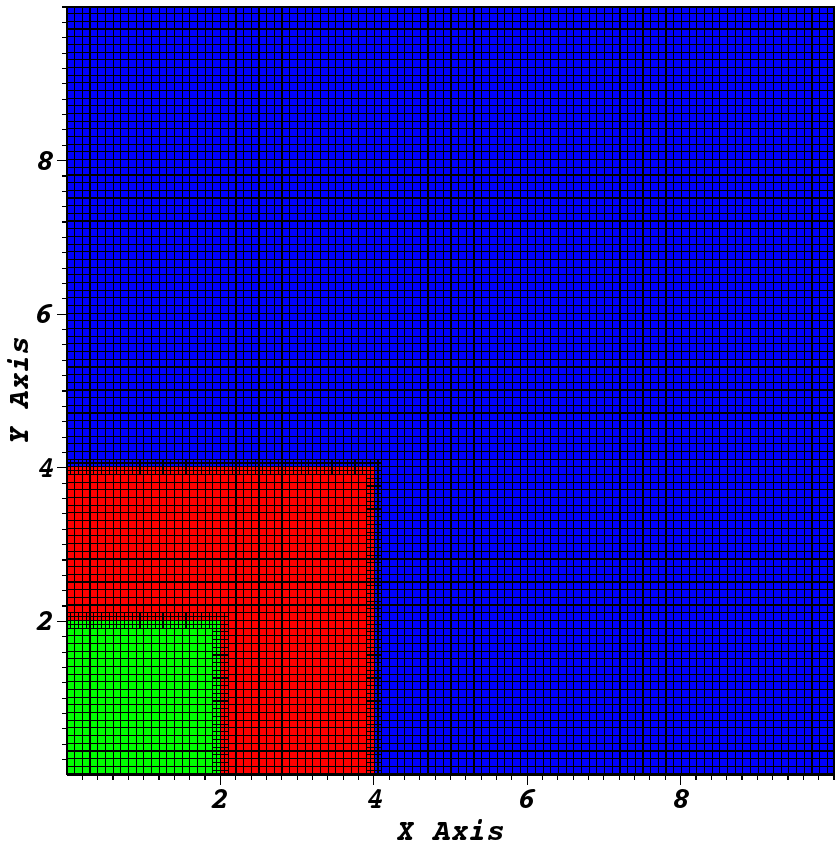
\includegraphics[width=6cm]{zone_amr}
    \caption{Material regions}
%    \label{mat_amr}
  \end{subfigure}
  \begin{subfigure}{0.75\textwidth}
    \centering
    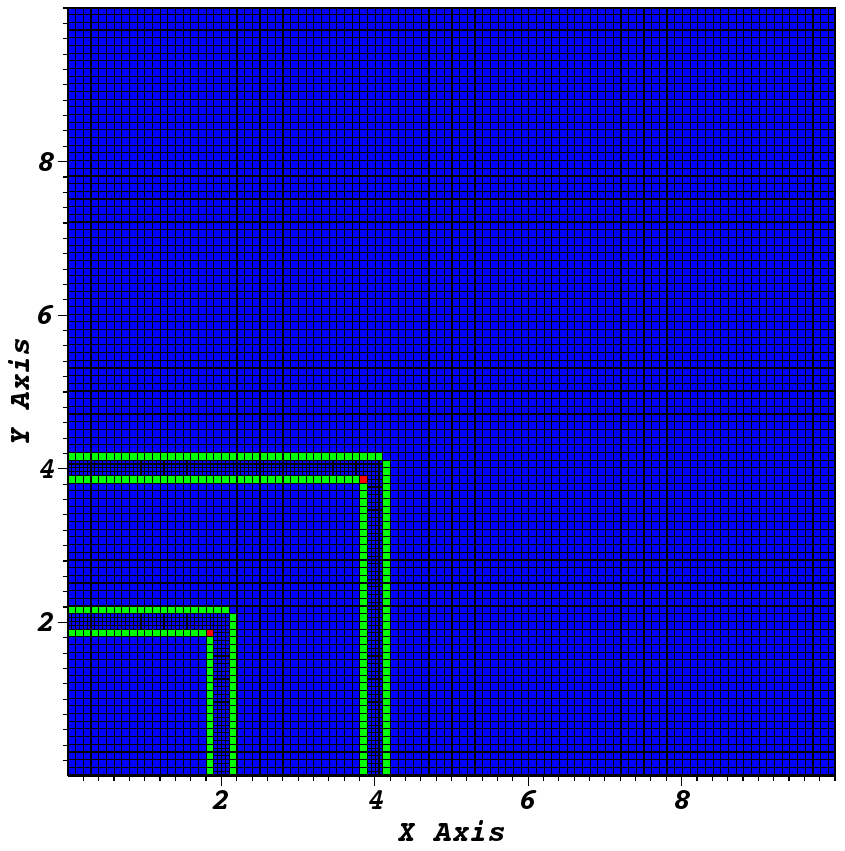
\includegraphics[width=6cm]{polygon_amr}
    \caption{Polygons distribution (the blue cells are quadrilaterals, the green cells are pentagons, and the red cells are hexagons)}
%    \label{fig_pol_dist}
  \end{subfigure}
  \caption{AMR-like test domain}
\end{figure}
%
\begin{table}
  \begin{center}
    \caption{Material properties, AMR-like test problem}
    \begin{tabular}{|c|c|c|c|}
      \hline
      & Inner region & Intermediate region & Outer region  \\ \hline
    $\Sigma_t$ $(cm^{-1})$ & 1.5  & 1.0 & 1.0 \\
    $\Sigma_s$ $(cm^{-1})$ & 1.44 & 0.9 & 0.3 \\
  Source $(cm^{-3}s^{-1})$ & 1.0  & 0.0 & 0.0 \\
      \hline
    \end{tabular}
    \label{prop_amr}
  \end{center}
\end{table}

where the blue cells are quadrilaterals, the green cells are pentagons, and
the red cells are hexagons. This mesh is typical of a mesh obtained after one 
level of adaptive mesh
refinement (the cells at the interface of different materials have been refined
once). We see that instead of introducing hanging nodes, we have introduced
pentagons and hexagons in the mesh.
\begin{table}[H]
  \caption{Comparison of preconditioners on AMR mesh}
  \begin{center}
    \begin{tabular}{|c|c|c|c|c|c|c|}
      \hline
       & No-DSA & CG & PCG-SGS & PCG-ML/U & PCG-ML/MIS & AGMG \\
      \hline
   SI iterations & 184     & 19      & 19       & 19      & 19       & 19 \\
Precond init (s) & NA      & NA      & 0.043463 & 0.358002 & 1.19301 & 0.0111\\
MIP calculation (s) & NA   & 48.1908 & 81.0992  & 25.2699 & 25.0699  & 
      2.56198\\
   CG iterations & NA      & 11300   & 4734     & 361     & 361      & 264 \\
     Total calculation (s) & 802.985 & 138.825 & 172.423  & 116.018 & 116.517  &
      94.1963\\
      \hline
    \end{tabular}
    \label{table_amr}
  \end{center}
\end{table}

\subsubsection{High aspect ratio grids}
%%%%%%%%%%%%%%%%%%%%%%%%%%%%%%%%%%%%%%%%%%%%%%%%%%%%%%%%%%%%%%%%%%%%%%%%%%%%%%%%%%

In these last two examples, a square domain  of $100cm \times 100cm$ with vacuum boundaries
is employed. There are 10,000 cells (thus, 40,000 degrees of freedom). Again, the relative 
tolerance on SI is $10^{-8}$ and the relative tolerance for CG is $10^{-10}$. 
An $S_8$ GLC angular quadrature is used. $\Sigma_t = 1cm^{-1}$, $\Sigma_s = 0.999cm^{-1}$,
and the source is $1n/(cm^3s)$. 
In the first run, the domain is discretized using 100 subdivisions of the $x$ and $y$
axes, i.e., 10,000 square cells with an aspect ratio of one. In the second run, 
the domain is discretized using 1,000 subdivision along $x$ and 10 along $y$ 
(the aspect ratio is then 100).
%
As expected, solving the MIP-DSA equations requires more CG iterations when the aspect
ratio increases. PCG-ML/U and PCG-ML/MIS are significantly more affected by the
increase in the aspect ratio than the other methods. AGMG is the least
affected by the change of aspect ratio and is again the best performing
preconditioner.
%
\begin{table}[!htbp]
  \caption{Comparison of preconditioners on rectangular grid with an aspect
  ratio of 1}
  \begin{center}
    \begin{tabular}{|c|c|c|c|c|c|c|}
      \hline
       & No-DSA & CG & PCG-SGS & PCG-ML/U & PCG-ML/MIS & AGMG \\
      \hline
      SI iterations & 7311      & 21      & 21      & 21       & 21      & 21 \\
   Precond init (s) & NA        & NA      & 0.01422 & 0.051373 & 1.13144 &
      0.044 \\
MIP calculation (s) & NA        & 32.3825 & 73.8422 & 24.0707  & 25.0065 &
      1.7114 \\
      CG iterations & NA        & 8363    & 4853    & 376      & 375     &
      221\\
Total calculation (s) & 7356.96 & 56.8993 & 98.2609 & 50.1247  & 51.5396 &
      25.9306 \\
      \hline
    \end{tabular}
    \label{table_ar_1}
  \end{center}
\end{table}
%
\begin{table}[!htbp]
  \caption{Comparison of preconditioners on rectangular grid with an aspect
  ratio of 100}
  \begin{center}
    \begin{tabular}{|c|c|c|c|c|c|c|}
      \hline
       & No-DSA & CG & PCG-SGS & PCG-ML/U & PCG-ML/MIS & AGMG \\
      \hline
      SI iterations & 7304    & 24      & 24        & 24       & 24      & 24 \\
   Precond init (s) & NA      & NA      & 0.0164239 & 0.362463 & 1.03128 & 0.052 \\
MIP calculation (s) & NA      & 372.227 & 742.902   & 941.06   & 922.258 &
      6.93176 \\
      CG iterations & NA      & 84802   & 43466     & 14180    & 13896   & 821 \\
Total calculation (s) & 9035.6 & 414.301 & 784.77   & 985.796  & 966.77  &
      44.7032 \\
      \hline
    \end{tabular}
    \label{table_ar_100}
  \end{center}
\end{table}                  

\section{Conclusions} \label{sec_conc}


% bibliography
\bibliographystyle{unsrt}
\bibliography{biblio}

\end{document}

